\section{Data Construction Details}

\begin{figure*}[ht]
    \centering
    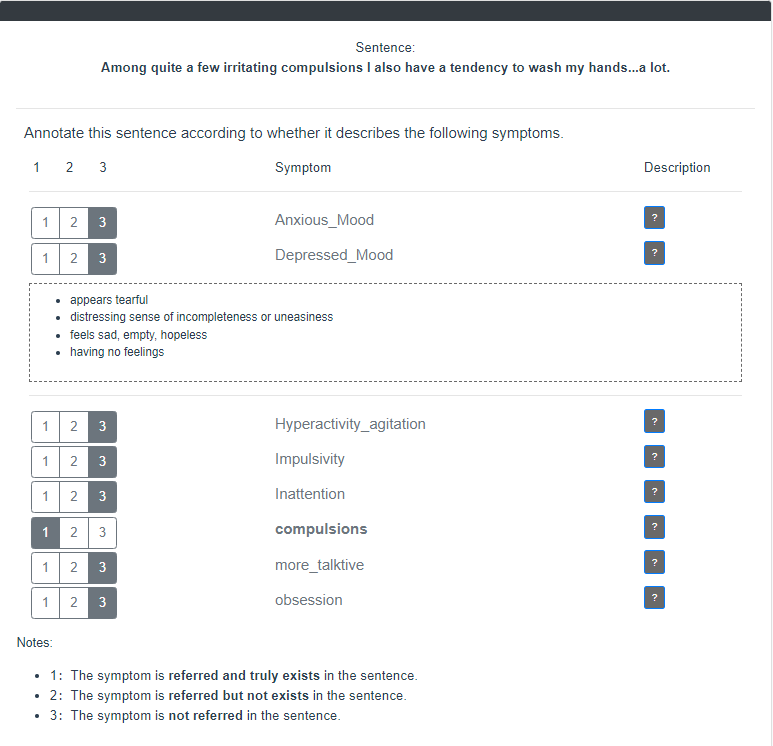
\includegraphics[width=1.8\columnwidth]{figures/anno_interface.png}
    \caption{Screenshot of the annotation interface.}
    \label{fig:anno_interface}
\end{figure*}

\subsection{Candidate Selection Algorithm}
\label{apd:cand}

Previous attempts to establish symptom annotation dataset \citep{mowery2017understanding} have shown that the distribution of different symptoms can be highly unbalanced, with many classes having too few positive samples to train a plausible classifier. On the other hand, we found in our preliminary annotations that it's hard to achieve high agreement on atypical expressions of symptoms. Therefore, to encourage a more balanced symptom distribution, while retrieving the most typical symptom posts for high annotation agreement, we designed a priority queue based algorithm for the selection of candidate posts with embedding similarity (\S \ref{sec:data_retrieval}):
\begin{enumerate}
    \item For the annotation of a disease $d$, we set up a queue with max capacity of 300 sentences for each symptom of $d$
    \item For each sentence $x$ in $d$'s related subreddits, and each symptom $s$ of $d$, we estimate the $x$'s relevance to $s$ with its max similarity with all sub-symptoms of $s$. We add $x$ into the queue of $s$, if it is not full, or $x$'s relevance is larger than the minimum one in $s$
    \item We aggregate the sentences from all queues, and perform deduplication with MinHash and Local Sensitive Hashing (LSH) \citep{leskovec2020mining} to eliminate identical or similar sentences. The remaining posts will be used as the annotation candidates for $d$.
\end{enumerate}

Since we only use sentences with the highest estimated relevance to symptoms, the selected posts tend to show more typical symptom expressions. The equal size of each symptom queue can further alleviate the class imbalance problem (see class distribution in Table \ref{tab:symp_count}) (but not totally eliminate it, because of the error of relevance approximation, the potential overlapping between queues and the inherent unbalanced distribution with in the original posts.)

\subsection{Status Annotation}

Initially, the symptom status is annotated on the basis of each symptom in a sentence. The reason is that a sentence can express multiple symptoms with different status. For example, in ``I don't have insomnia any more, but I'm still depressed.'', the status of the previous symptom is negative while that of the latter is positive. However, after annotation, we find that the negative status annotation for each symptom is scarce. We then consider merging all symptom-level status into sentence-level. The motivation are two-folds. First, we observed that most sentences with negative status share similar characteristics like having negation words or being a question. Moreover, we found that the conflicts between status annotations of different symptoms in the same sentence is rare, accounting for only 2.8\% of the sentences. We thus set the sentence-level status as negative if there is any negative status annotation in its relevant symptoms. If not specified, the PsySym discussed in this paper refers to the version with sentence-level status labels.

\subsection{Quality Control}

\begin{table}[ht]
    \small
    \centering
    \begin{tabular}{cc}
    \hline
    Disease & \# of sentences   \\
    \hline
    ADHD & 528\\
    Anxiety & 2822\\
    Bipolar Disorder & 1131 \\
    Depression & 1433\\
    Eating Disorder & 907\\
    OCD & 449\\
    PTSD & 1284\\
    \hline
    \end{tabular}
    \caption{Annotated number of sentences for each disease.}
    \label{tab:disease_count}
\end{table}

\begin{table}[ht]
    \small
    \centering
    \begin{tabular}{m{4.8cm}m{0.9cm}m{0.9cm}}
    \hline
    Symptom & \#Positive & $\kappa$ \\
    \hline
    Anxious Mood 	&	1790	&	0.736 	\\
    Autonomic symptoms	&	571	&	0.786 	\\
    Cardiovascular symptoms	&	506	&	0.937 	\\
    Catatonic behavior	&	231	&	0.668 	\\
    Decreased energy tiredness fatigue	&	250	&	0.728 	\\
    Depressed Mood	&	846	&	0.637 	\\
    Gastrointestinal symptoms	&	340	&	0.943 	\\
    Genitourinary symptoms	&	260	&	0.951 	\\
    Hyperactivity agitation	&	277	&	0.603 	\\
    Impulsivity	&	157	&	0.776 	\\
    Inattention	&	401	&	0.801 	\\
    Indecisiveness	&	151	&	0.779 	\\
    Respiratory symptoms	&	464	&	0.916 	\\
    Suicidal ideas	&	287	&	0.915 	\\
    Worthlessness and guilty	&	291	&	0.614 	\\
    avoidance of stimuli	&	78	&	0.495 	\\
    compensatory behaviors to prevent weight gain	&	423	&	0.869 	\\
    compulsions	&	168	&	0.767 	\\
    diminished emotional expression	&	179	&	0.547 	\\
    do things easily get painful consequences	&	316	&	0.804 	\\
    drastical shift in mood and energy	&	425	&	0.889 	\\
    fear about social situations	&	415	&	0.938 	\\
    fear of gaining weight	&	257	&	0.747 	\\
    fears of being negatively evaluated	&	127	&	0.606 	\\
    flight of ideas	&	237	&	0.810 	\\
    intrusion symptoms	&	260	&	0.720 	\\
    loss of interest or motivation	&	181	&	0.676 	\\
    more talktive	&	165	&	0.647 	\\
    obsession	&	433	&	0.748 	\\
    panic fear	&	419	&	0.808 	\\
    pessimism	&	332	&	0.707 	\\
    poor memory	&	264	&	0.854 	\\
    sleep disturbance	&	320	&	0.852 	\\
    somatic muscle	&	428	&	0.879 	\\
    somatic symptoms others	&	347	&	0.723 	\\
    somatic symptoms sensory	&	258	&	0.777 	\\
    weight and appetite change	&	486	&	0.794 	\\
    Anger Irritability	&	427	&	0.841 	\\
    \hline
    \end{tabular}
    \caption{Number of positive samples (multiple annotations of a sentence aggregated) and Fleiss's $\kappa$ of symptoms}
    \label{tab:symp_count}
\end{table}


\begin{table}[h]
    \small
    \centering
    \begin{tabular}{lc}
    \hline
    Disease          & \# Users \\
    \hline
    Depression       & 3105         \\
    Anxiety          & 2239         \\
    Autism           & 716         \\
    ADHD             & 2374         \\
    Bipolar Disorder & 1366         \\
    OCD              & 753          \\
    PTSD             & 391          \\
    Schizophrenia    & 345          \\
    Eating Disorder  & 138          \\
    \hline
    \end{tabular}
    \caption{Number of users suffering from each disease in the disease detection dataset.}
    \label{tab:disease_detect_count}
\end{table}

\paragraph{Score Calculation} One core component of our quality control measures is the annotation quality score. Given the annotations and references (judgment from the authors), the quality score is calculated as the symptom-level $F_{\beta}$ score between them. The $\beta$ is set to 2 to put more emphasis on recall. 

The score is used in several phases of the annotation \ref{sec:data_annotation}. In \textit{Screening Tests}, the annotators need to achieve above 75 score to be qualified to conduct further annotation. We will also calculate the score in \textit{Sampling Inspection}, and reject all annotations in the checking batch if the score is below 60. To motivate accurate annotation, the volunteers will be rewarded with higher subsidy for high scores achieved according to our inspection.

\paragraph{Annotation Interface} The annotation interface is a customized webpage with many designs to promote efficient and accurate annotations. First, the annotator will be enter a disease description page, where all symptoms and their descriptions are shown for annotators to get familiar with. They will then enter the annotation page (Figure \ref{fig:anno_interface}). All symptom names are shown in list below the sentence to annotate. Annotators can click on the question mark beside the symptom to expand its descriptions, which can serve as a quick reminder. We will also make a symptom bold, if the sentence hit any keywords in the symptom descriptions, which can help the annotators quickly focus on likely classes, and also prevent them from missing annotations in case the annotators are unaware of some items in the symptom descriptions. 

\subsection{Detailed Data Statistics}
\label{apd:stats}

We show the number of annotated sentences for each disease in Table \ref{tab:disease_count}, where diseases with more symptoms will have more annotations. We also show the number of annotations and the inter-annotator agreement by each symptom in Table \ref{tab:symp_count}. It can be seen that almost all symptom classes received reasonable amount of annotations, and have high agreement, indicating the effectiveness of proposed annotation framework to guarantee the quality of PsySym. We provide more examples in Table \ref{tab:more_label_example}.

For the disease detection dataset (\S \ref{sec:data_disease}), we also provide the number of users suffering from each disease in Table \ref{tab:disease_detect_count}. The distribution of the 9 diseases are similar to SMHD \citep{cohan2018smhd}.

\section{Detailed Experimental Settings}
\label{apd:settings}

\begin{table*}[t]
    \centering
    \begin{tabular}{lcccc}
    \hline
    Disease           & TF-IDF & BERT  & Symp  & Symp (Reweighting) \\ \hline
    Depression        & 68.95  & 71.58 & 66.67 & 69.88              \\
    Anxiety           & 66.48  & 71.08 & 71.82 & 71.39              \\
    ADHD              & 59.55  & 60.05 & 60.14 & 60.45              \\
    Bipolar Disorder  & 66.67  & 43.56 & 67.76 & 68.82              \\
    OCD               & 26.09  & 44.83 & 48.33 & 56.52              \\
    PTSD              & 30.43  & 27.45 & 48.48 & 45.9               \\
    Eating Disorder   & 11.11  & 37.04 & 52.17 & 46.15              \\ \hline
    Autism            & 30.23  & 49.59 & 35.64 & 37.04              \\
    Schizophrenia     & 34.04  & 57.97 & 48.15 & 57.63              \\ \hline
    Mean (7 Diseases) & 47.04  & 50.80 & 59.34 & \textbf{59.87}     \\
    Mean (9 Diseases) & 43.73  & 51.46 & 55.46 & \textbf{57.09}     \\ \hline
    \end{tabular}
    \caption{MDD results by disease. We distinguish the 7 disease types included in PsySym (upper) and the remaining two (lower), and calculate the average performance with 7 and 9 diseases.}
    \label{tab:mdd_by_disease}
\end{table*}

For all models, we empirically set hyperparameters following existing implementations and previous works without fine-tuning them for optimized performance. Specifically, we use a learning rate (lr) of 3e-4, max sequence length of 64 for BERT and MBERT models used for symptom relevance judgment and status inference. For the CNN model used in mental disease detection, the structure is identical to that of \citet{nguyen2022improving}, the lr is 0.01 when using symptom features only and 0.003 when using BERT embeddings or the combined features. The posting list will be truncated to preserve the earliest 256 posts at most. We also employ early-stopping with a patience of 4 epochs according to validation performance to prevent overfitting. For efficiency of inference on the MDD dataset with large amount of posts, we use bert-tiny \footnote{\url{https://huggingface.co/prajjwal1/bert-tiny}} models trained on PsySym to extract the symptom and status features, whose performance is close to the best performing MBERT model (AUC=98.80, F1=62.28 for relevance judgement with control posts and MAE=0.1509 for status inference). For the multi-task learning of multiple symptoms, the losses of each classes are the simple arithmetic mean of them without weighting. 

For each post, we conduct several preprocessing steps. First, they are split into sentences with \textit{blingfire}\footnote{\url{https://github.com/microsoft/BlingFire}}. We will then eliminate sentences like ``[Removed]''. We also use regular expressions to detect the hyperlink format like ``[anchor text](web url)'', and transform it into only anchor text.

\section{Detailed Disease Detection Results}
\label{apd:mdd_results}

We show the MDD performance of different methods on disease level in Table \ref{tab:mdd_by_disease}. It can be seen that the proposed symptom-based methods perform slightly worse than BERT on the 2 diseases not included in PsySym, which is reasonable. When comparing only the 7 PsySym diseases the advantage of Symp over BERT is even more significant, which further demonstrate the strength of the proposed method. We also observe a more significant improvement on diseases with fewer positive samples like OCD, PTSD and Eating Disorder, suggesting the usefulness of symptom knowledge for the MDD in low-resource scenarios.

\section{Per-Symptom Analysis}

\begin{figure*}[ht]
    \centering
    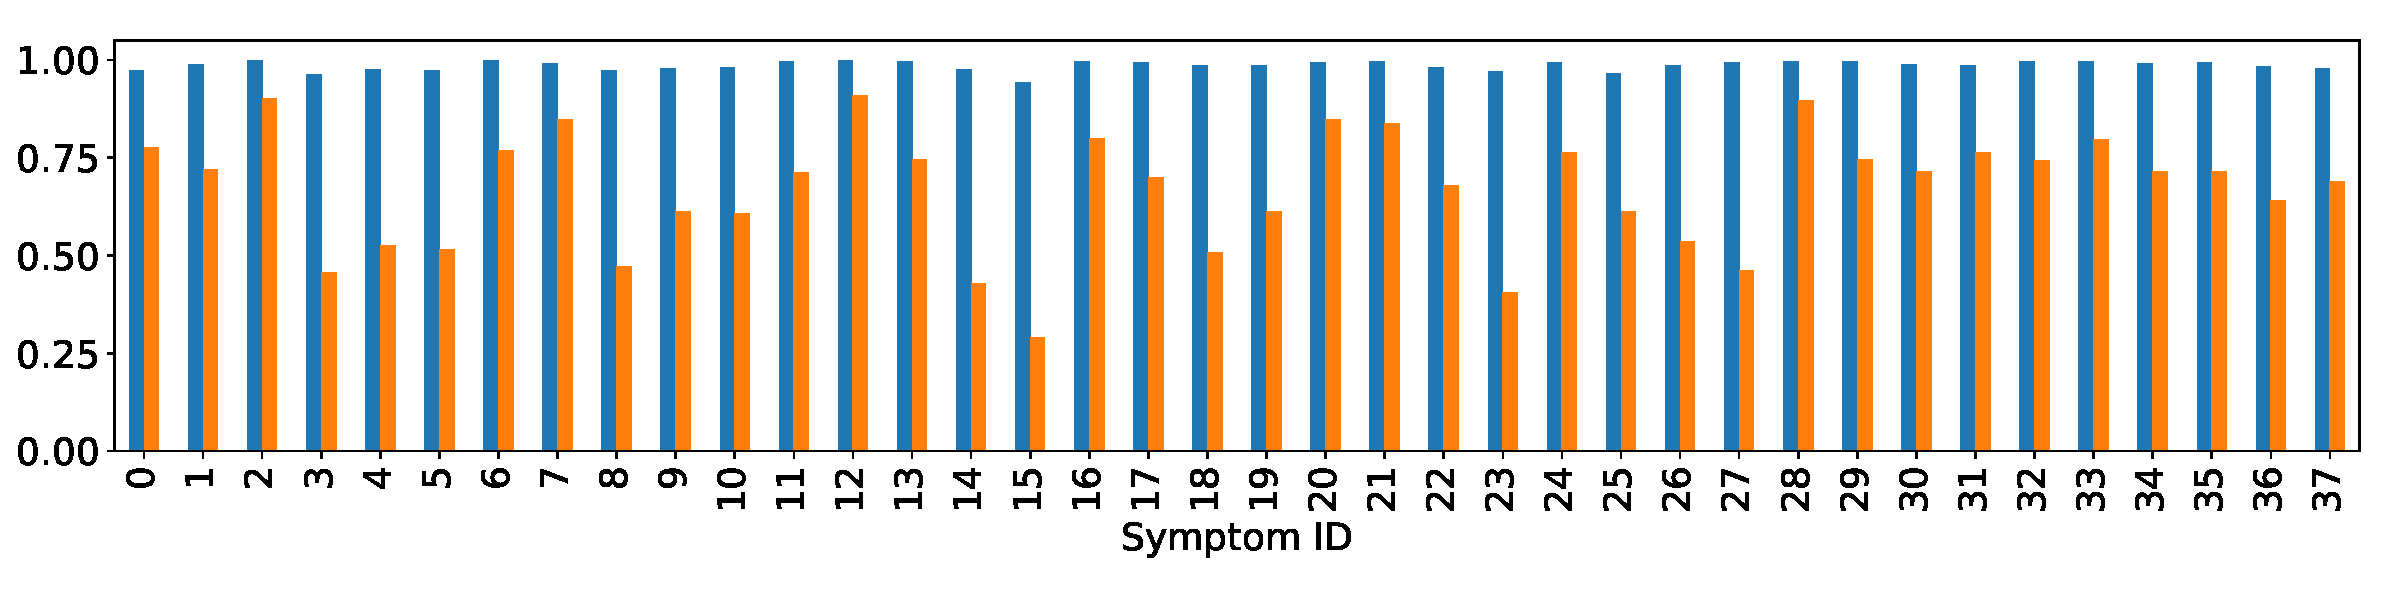
\includegraphics[width=2.0\columnwidth]{figures/Symptom_AUC_F1_Multi_disease.pdf}
    \caption{Identification performance of each symptom with the MBERT (label enhance) model trained on data with control posts (\S \ref{sec:relevance_exp}). The blue bar shows the AUC while the orange bar shows F1, and Symptom ID follows the order of Table \ref{tab:symp_count}.}
    \label{fig:Symptom_AUC_F1_Multi_disease}
\end{figure*}

\begin{table*}[h]
    \small
    \centering
    \begin{tabular}{|l|l|l|}
    \hline
    Post                                        & Symptom(s)                & $P_{uncertain}$ \\ \hline
    \begin{tabular}[c]{@{}l@{}}I believe most ADHDers struggle in conversation:  \\ * Impulsivity makes it hard for us to wait our turn while someone is talking\end{tabular} &
      \begin{tabular}[c]{@{}l@{}}Hyperactivity; Impulsivity; \\ Inattention\end{tabular} &
      1/3 \\ \hline
    Venting about stomach aches and no eating. & Gastrointestinal Symptoms & 0            \\ \hline
    \begin{tabular}[c]{@{}l@{}}I don't want to use laxatives and diuretics \\ because I know how bad they are to your body.\end{tabular} &
      \begin{tabular}[c]{@{}l@{}}Compensatory behaviors to\\ prevent weight gain\end{tabular} &
      1 \\ \hline
    \end{tabular}
    \caption{More example of the PsySym dataset. $P_{uncertain}$ is the portion of annotators who labeled one of the symptoms as uncertain. }
    \label{tab:more_label_example}
\end{table*}

We further conduct analysis on the identification performance of each symptom to gain insights on their varied difficulty. We show the classification AUC and F1 (given threshold=0.5) on these symptoms with our best performing model MBERT (label enhance) model trained on data with control posts in Figure \ref{fig:Symptom_AUC_F1_Multi_disease}. We can see that AUC and F1 are strongly correlated (Pearson's $r$=0.78), and from F1 we can clearly see that many symptom classes still have abundant room for improvement. Inter-annotator agreement ($\kappa$ in Table \ref{tab:symp_count}) can also affect the identification performance, with Pearson's $r$ between $\kappa$ and F1 = 0.86. This is because some classes are inherently more ambiguous than others, which makes both human agreement and model classification difficult. For example, as the first row of Table \ref{tab:more_label_example} shows, the symptom ``Hyperactivity'' and ``Inattention'' do not have explicit terms in the post and needs to be inferred, which makes them difficult to identify. However, we can easily find ``Gastrointestinal Symptoms'' in the second row with the phrase ``stomach aches''. 